% !TeX root = ../main.tex

\chapter{Path Integral}

\begin{enumext}[label = *]
  \item What is a path? --- $x(t)$.
  $\phi: I \equiv [0,1] \to R^d$, $t \in I$, $t_i = 0$, $t_f = 1$.
  
  $I \to R^d$, $I \to M$, $R^{d+1} \to M$: $\phi \in$ Function space.
  ($d + 1$: dimension and time)
  \item What to integrate? $\sum_\phi G[\phi]$. $G: V \to \mathbb C$.

  E.g.: $F[x(t)] \to f(x_1,x_2, \cdots x_N) \leftarrow f(x) = ax^m $
  \item Quantization Schemes: Canonical Quantization $\Leftrightarrow$ Path Integral

  States \& Operators.

  In qm, $\braket<O_1,O_2> \to$ trasition amplitudes, propagate.

  Something like $\int \mathcal D\phi G[\phi]$ will eventually produce something like $\braket<O_1,O_2>$.
\end{enumext}

\section{Compare Quantum with Classical Limit}

\begin{enumext}[label = (\alph*)]
  \item Quantum
    \[
      \hat U(t_f,t_i) = \mathbbm 1 + \ab(-\frac\iu\hbar) \int_{t_i}^{t_f} \d t_1 \hat H(t_1)
    + \ab(-\frac\iu\hbar)^2 \int_{t_i}^{t_f} \d t_1 \int_{t_i}^{t_1} \d t_2   \hat H(t_1) \hat H(t_2) + \cdots
    \]
    Problem: Discontinuous!
    The Hamiltonian actually shall be ``local''.
    One of $H$ act on state, it could not jump.
    \begin{center}
      \begin{minipage}{.42\linewidth}
        \centering
      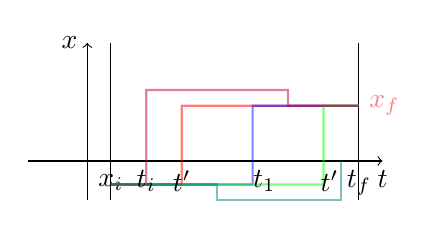
\begin{tikzpicture}[xscale = 1.5]
        \draw (.2,-.5) node [ above ] {$x_i$} --++ (0,2);
        \draw (2.3,-.5) --++ (0,2);
      \draw [->] (-.5,0) -- (2.5,0) node [below] {$t$};
      \draw [->] (0,-.5) -- (0,1.5) node [left] {$x$};
      \draw [thick, opacity = .5, red] (.2,-.3) --++ (.6,0) --++ (0,1) -- (2.3,.7) node [right] {$x_f$};
      \draw [thick, opacity = .5, blue] (.2,-.3) --++ (1.2,0) --++ (0,1) -- (2.3,.7);
      \draw [thick, opacity = .5, green] (.2,-.3) --++ (1.8,0) --++ (0,1) -- (2.3,.7);
      \draw [thick, opacity = .5, purple] (.2,-.3) --++ (.3,0) --++ (0,1.2) --++ (1.2,0) --++ (0,-.2) -- (2.3,.7);
      \draw [thick, opacity = .5, teal] (.2,-.3) --++ (.9,0) --++ (0,-.2) --++ (1.05,0) --++ (0,.5);
      \node [below] at (.5,0) {$t_i$}
       node [below] at (.8,0) {$t'$}
       node [below] at (1.5,0) {$t_1$}
       node [below] at (2.05,0) {$t'$}
       node [below] at (2.3,0) {$t_f$};
      \end{tikzpicture}
      \end{minipage}
      \hspace*\fill
      It should be
      \hspace*\fill
      \begin{minipage}{.42\linewidth}
        \centering
      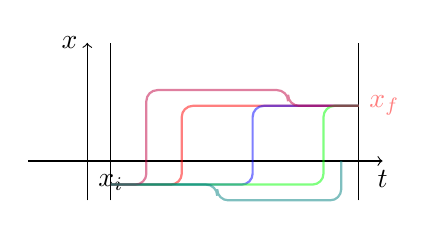
\begin{tikzpicture}[xscale = 1.5]
        \draw (.2,-.5) node [ above ] {$x_i$} --++ (0,2);
        \draw (2.3,-.5) --++ (0,2);
      \draw [->] (-.5,0) -- (2.5,0) node [below] {$t$};
      \draw [->] (0,-.5) -- (0,1.5) node [left] {$x$};
      \draw [rounded corners, thick, opacity = .5, red] (.2,-.3) --++ (.6,0) --++ (0,1) -- (2.3,.7) node [right] {$x_f$};
      \draw [rounded corners, thick, opacity = .5, blue] (.2,-.3) --++ (1.2,0) --++ (0,1) -- (2.3,.7);
      \draw [rounded corners, thick, opacity = .5, green] (.2,-.3) --++ (1.8,0) --++ (0,1) -- (2.3,.7);
      \draw [rounded corners, thick, opacity = .5, purple] (.2,-.3) --++ (.3,0) --++ (0,1.2) --++ (1.2,0) --++ (0,-.2) -- (2.3,.7);
      \draw [rounded corners,  thick, opacity = .5, teal] (.2,-.3) --++ (.9,0) --++ (0,-.2) --++ (1.05,0) --++ (0,.5);
      \end{tikzpicture}
      \end{minipage}
    \end{center}
    $U$ can be decompose like
    \[
      \hat U(t_f,t_i) = \hat U(t_f,t_{N-1}) \cdots \hat U(t_N,t_{N-1}) \cdots \hat U(t_i,)
    \]
    \item Path Integral
    \begin{align*}
      & U(x_f,t_f;x_i,t_i) \equiv \braket<x_f|\hat U(t_f,t_i)|x_i>\\
    = & \int \d x_i \cdots \d x_{N-1} \braket<x_f |\hat U(t_f,t_{N-1})|x_{N-1}>
    \braket<x_{N-1}|\hat U(t_{N-1},t_{N-2})|x_{N-2}> \cdots\\
    & \braket<x_n |\hat U(t_n,t_{n-1})|x_{n-1}> \cdots \braket<x_1|\hat U(t_1,t_i)|x_i>
    \end{align*}
    Basically, we can write the time evolution
    \[
      U(x_n,t_n;x_{n-1},t_{n-1}) = \braket<x_n |\hat U(t_n,t_{n-1})|x_{n-1}> \approxeq \braket<x_n|\upe^{-\frac\iu\hbar\hat H(t_n) \delta t}|x_{n_1}>
    \]
    it's vavid when $\delta t$ is very small.
    Insert a complete basis
    \begin{align*}
      U(x_n,t_n;x_{n-1},t_{n-1}) & \approxeq
      \int \d p_n \braket<x_n|\upe^{-\frac\iu\hbar\hat H(t_n) \delta t}|p_n>\braket<p_n|x_{n_1}>\\
      & = \frac1{2\pi\hbar} \int \d p_n \upe^{\frac\iu\hbar}[p_n(x_n - x_{n-1}) - H(x_n,p_n,t_n)\delta t]
    \end{align*}
  Consider
  \[
    \int \prod_{n=1}^{N-1} \d x_n \int\prod_{n=1}^N \d p_n
  \]
  which is so called ``path'': in phase space path integral.
  (Consider the time is divided in many pieces).
  Then $U(x_n,t_n;x_{n-1},t_{n-1})$ can be
  \[
    U(x_n,t_n;x_{n-1},t_{n-1}) = \int \d p_n \upe^{\frac{\iu}{\hbar} [p_n\dot x_n - \frac{p_n^2}{2m} - V(x_n,t_n)]\delta t}
  = \ab(\frac m{2\pi\iu\hbar\delta t})^{1/2} \upe^{\frac\iu\hbar[\frac12m\dot x_n^2 - V(x_n,t_n)]\delta t}
  \]
  where $\dot x_n = \frac{x_n - x_{n-1}}{\delta t}\big|_{\delta t \to 0}$,
  and $\frac12m\dot x_n^2 - V(x_n,t_n)$ is the Lagrangian $\mathcal L(x_n,\dot x_n,t_n)$.
  Eventually,
  \[
    U(x_f,t_f;t_i,t_i) = \ab(\frac m{2\pi\iu\hbar\delta t})^{N/2}
    \int \prod_{n=1}^{N-1} \d x_n \upe^{\frac\iu\hbar \sum_{n=1}^{N-1}}
    \mathcal L(x_n,\dot x_n,t_n) \delta t
  = \int \mathcal D x(t) \upe^{\frac\iu\hbar\mathcal S[x]}
  \]
  where $\mathcal D = \int \prod_{n=1}^{N-1} \d x_n$,
  and $\mathcal S[x] \equiv \int_{t_i}^{t_f} \d t \mathcal L(x,\dot x,t)$ ($N \to \infty$).
  In summary, we obtain
\begin{equation}
  U(x_f,t_f;x_i,t_i) \equiv \int \mathcal D x(t) \upe^{-\frac\iu\hbar \mathcal S[x(t)]}
\end{equation}
  where $x(t_i) = x_i$ and $x(t_f) = x_f$.
  \item Classical
  \[
    \hat H(t_n) = \frac{\hat p^2}{2m} + V(\hat x,t_n)
  \]
  Using $\upe^{-\iu\hat H\delta t} \approxeq 1 - \iu\hat H\delta t$.
  Then, we can simply evalute $\braket<x_n|\hat H|p_n>$.
  \[
    \braket<x_n|\upe^{-\frac\iu\hbar\hat H(t_n)\delta t}|p_n>
  = \upe^{-\frac\iu\hbar H(x_n,p_n,t_n)\delta t} \braket<x_n|p_n>
  = \upe^{-\frac\iu\hbar H(x_n,p_n,t_n)\delta t + \frac\iu\hbar p_nx_n}
  \]
  where $H(x_n,p_n,t_n) = \frac{p_n^2}{2m} + V(x_n,t_n)$.
  \hrule \newpage
  Principle of Least Action, EOM determines $x_c(t)$.
  The equation can be derived by
  \begin{equation}
    \delta \mathcal S = 0,\qq{or} (\delta_x\mathcal S)[\eta] = 0, \forall \eta
  \end{equation}
  we fix the initial $(x_i,t_i)$ and the final $(x_f,t_f)$. Consider the other path $x'(t)$, the different is $\eta(t)$.
  Starting from the action
  \begin{equation}
    \mathcal S[x(t)] = \int_{t_i}^{t_f} \d t \mathcal L(x(t), \dot x(t), t)
  \end{equation}
  On another path, the action is
  \[
    \mathcal S[x_c + \eta_c] = \int_{t_i}^{t_f} \d t \mathcal L(x_t + \eta_t, \dot x_t + \dot \eta_t,t)
  = \int_{t_i}^{t_f} \d t \ab[\mathcal L(x_t,\dot x_t,t) + \pdv{\mathcal L}{x_t} \eta t
  + \pdv{\mathcal L}{\dot x_t} \dot \eta_t + \mathcal O(\eta^2)]
  \]
  where
  \[
    \int_{t_i}^{t_f} \d t \ab(\pdv{\mathcal L}{x_t} \eta t
  + \pdv{\mathcal L}{\dot x_t} \dot \eta_t)
  \]
  is so-called \emph{functional derivative}\footnote{From functional space to functional space: $V^* \to V^*$.}: $(\delta_x \mathcal S)[\eta]$.
  Apply the partition integration
  \[
    (\delta_x\mathcal S)[\eta] = \pdv L{\dot x_t} \eta_t \big|_{t_i}^{t_f}
  + \int_{t_i}^{t_f} \d t\ab(\pdv{\mathcal L}{x_t} - \odv*{\pdv{\mathcal L}{\dot x_t}}t)\eta_t
  \]
  since $\eta(t_i) = \eta(t_f) = 0$, so
  \[
    (\delta_x\mathcal S)[\eta] = \int_{t_i}^{t_f} \d t\ab(\pdv{\mathcal L}{x_t} - \odv*{\pdv{\mathcal L}{\dot x_t}}t)\eta_t
  \]
  the integral kernel can be converted to
  \[
    \ab(\pdv{\mathcal L}{x_t} - \odv*{\pdv{\mathcal L}{\dot x_t}}t)\eta_t
  = \braket<\pdv{\mathcal S}{x_i}|\eta>
  \]
  \underline{For $\forall \eta$}, the integral kernel should be zero
  \begin{equation}
    \pdv{\mathcal L}{x_t} - \odv*{\pdv{\mathcal L}{\dot x_t}}t = 0
  \end{equation}
  it's so-called the \emph{Euler-Lagrangian Equation}.
\end{enumext}

Let's talk more about functional derivative.
\[
  (\delta^{(n)}_x\mathcal S)[\eta] = \odv[n]{\mathcal S[x(t) + \epsilon\eta(t)]}\epsilon\bigg|_{\epsilon=0}
\]
the $x$ is supposed to ``where we take the derivative''.
$\mathcal S[x(t) + \epsilon\eta(t)]$ gives a number, but the number is depend on $\epsilon$. So we can define
\[
  \odv[n]{f_{x,\eta}(\epsilon)}{\epsilon} = \mathcal S[x(t) + \epsilon\eta(t)]
\]
\textbf{Quiz}.
Let's try an example.
\[
  \mathcal L(x(t), \dot x(t)) = \frac12m\dot x^2 - \frac12 m\omega^2x^2
\]
Try to find $\delta_x^{(0)}\mathcal S[\eta]$,
$\delta_x^{(1)}\mathcal S[\eta]$,
$\delta_x^{(2)}\mathcal S[\eta]$,
$\delta_x^{(3)}\mathcal S[\eta]$
using the definition.
(Solution: $\delta_x^{(0)}\mathcal S[\eta] = \mathcal S[x]$,
$\delta_x^{(1)}\mathcal S[\eta]$: $\ddot x = -\omega^2t$, $\delta_x^{(2)}\mathcal S[\eta] = 2\mathcal S[\eta]$, $\delta_x^{(> 2)}\mathcal S[\eta] = 0$.)

Let's try to write the Taylor expression of $\mathcal S[x + \eta]$
\begin{equation}
  \mathcal S[x + \eta] = \mathcal S[x + \eta]\big|_{\epsilon = 1} = f(\epsilon)_{x,\eta},
\end{equation}
then, just expand $f(\epsilon)_{x,\eta}$
\[
  \mathcal S[x + \eta] = f(0) + f'(0)\epsilon + \cdots + \frac1{n!}f^{(n)}(0) \epsilon^n + \cdots
\]
Concering $f^{(n)}_{x,\eta} = (\delta_x^{(n)} \mathcal S)[\eta]$, then
\begin{equation}
  \mathcal S[x + \eta] = (\delta^{(0)}\mathcal S)[\eta] + (\delta^{(1)}\mathcal S)[\eta] + \cdots + \frac1{n!}(\delta^{(n)}\mathcal S)[\eta]
= \ab(\upe^{\delta_x}\mathcal S)[\eta]
\end{equation}
\fbox{$\text{ELE} \to x_i(t)$}
\begin{equation}
  \upe^{\frac\iu\hbar\mathcal S[x+\eta]} = \upe^{\frac\iu\hbar(\mathcal S[x] + (\delta_x^{(0)}\mathcal S)[\eta] + \frac12(\delta_x^{(1)}\mathcal S)[\eta] + \cdots)}
\end{equation}
Since $\int \mathcal D\eta(t)$ taken the first order, then the other terms should vanish.
Since classical limit require $\hbar$ to be small.

\section{PI \& Sta. Mech.}

\paragraph{Review}
Starting from propagator
\[
  \braket<x_f|\hat U(t_f, t_i)|x_i> = \sum_{x(t)} \upe^{\iu S[x(t)]}
\]
Summing over all the functions (paths).
This is precisely the quantum interference
\begin{center}
  \begin{tikzpicture}
    \draw (0,0) node [below] {$t_i$} --++ (0,2) node [midway, left] {$x_i$};
    \draw (4,0) node [below] {$t_f$} --++ (0,2) node [near end, right] {$x_f$};
  \end{tikzpicture}
\end{center}
We can use a fancier symbol
\[
  \braket<x_f|\hat U(t_f, t_i)|x_i>
= \int_{x(t_{i,f}) = x_{i,f}} \mathcal D x(t) \upe^{\iu S[x(t)]}
\]
\paragraph{Statistics Mechanics}

Starting from the partition function
\begin{equation}
  Z = \sum_n \upe^{-\beta E_n} = \sum_{\fbox{\tiny ?}} \fbox ?
\end{equation}
$n$ means we sum over the \emph{microstates}: they are configuration.
\newcommand \circlespin[1]%
  {\mbox{\tikz{%
    \draw (0,0) circle (1ex);
    \draw [-stealth] (0,0) --++ (#1:1ex);
  }}}
\begin{example}
  A general picture about what are microstates and configurations.
  \begin{enumext*}[columns = 2]
    \item Two configurations: $\{\uparrow, \downarrow\}$.
    \item Four configurations: $\{\uparrow, \uparrow, \downarrow, \downarrow\}$
    \item(2) It can also a continous set, a circle, spin point to all possible orientation in a plane, the configuration space of the case.
    \[
      \{\circlespin{0}, \circlespin{45}, \circlespin{135}, \cdots\}
    \]
    \item(2) We can also have two objects, two circles cross to each others
    \[
      \{\} \approxeq S^1 \times S^1
    \]
    \item(2) About (Quantum) H.O.: $\{\circlespin{30}, \circlespin{-150}\}$ Something like a string, can be stationary. The shapes for the string can be also configurations.
    \item Oscillator: energy levels.
  \end{enumext*}
\end{example}
Recall the P.I. $\phi = x(t)$, Generalize it
\begin{align*}
  \mathbb I (\tikz[font = \tiny]{\draw (0,0) node [above] {$t_i$} -- (.5,0) node [above] {$t_f$};}) & \longrightarrow \mathbbm R (\{x\})\\
  \downarrow\\
  \mathbbm R^{d+1} (\mathbbm Z^{d+1}) & \longrightarrow M
\end{align*}
We can say we sum over the states, i.e., sum over different configurations
\[
  Z = \sum_\phi \upe^{-\beta E(\phi)}
\]
The configurations can be how these levels are occupied.
Concering the $\beta E$ term: Energy depends on the configuration, a kind of map, then it contribute to a Boltzman function.
\begin{enumext}[columns = 2]
  \item How the P.I. can be the P.F.
  \item How the P.F. can be something of P.I.
\end{enumext}
\[
  Z = \Tr \upe^{-\beta \hat H}
\]
\subsection{Analytic Continuation}

This somehow we go from P.I. to P.F.
We have a targest space $M$. From the $I$, between $t_i$ and $t_f$, mapping to the space $M$, where $t \in \mathbb R$.
And a complex plane $\mathbbm C$.
\begin{center}
  \begin{minipage}{.32\linewidth}
    \centering
    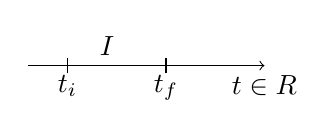
\begin{tikzpicture}
      \draw [->] (0,0) --++ (3,0) node [below] {$t \in \mathbbm R$};
      \node [below] at (.5,0) {$t_i$} node [below] at (1.75,0) {$t_f$}
       node [above] at (1,0) {$I$};
      \draw (.5,-.1) --++ (0,.2) (1.75,-.1) --++ (0,.2);
    \end{tikzpicture}
  \end{minipage}
  \hspace*\fill
  \textrightarrow The space $M$ \textleftarrow
  \hspace*\fill
  \begin{minipage}{.32\linewidth}
    \centering
    \begin{tikzpicture}
      \draw [->] (-.5,0) -- (2,0) node [below] {$t$};
      \draw [->] (0,-.5) -- (0,2);
      \node at (1,1) {$\mathbb C$} node at (.5,1.5) {$z$};
    \end{tikzpicture}
  \end{minipage}
\end{center}
\[
  \phi(t) \mapsto \phi(z) \phi(\tau)
\]
Map from a real axix to the target space,
map from the imaginary axis in the complex plane to the target space.
The property of the two maps really colse link together.

In summary: First, from $t$ to $z$, $t \mapsto z$,
then choose Z to be part of the imaginary axis or numbers, i.e., $z = -\iu\tau$. As the following examples
\begin{framed}
  \begin{multicols}{3}
  \begin{example}
    $t \mapsto z = -\iu\tau$
  \end{example}
  \begin{example}
    $\d t \mapsto -\iu\d\tau$
  \end{example}
  \begin{example}
    $\pdv*{}t \mapsto \iu \pdv*{}\tau$
  \end{example}
  \begin{example}
    $\pdv*\phi t \equiv \dot \phi \mapsto \iu \dot\phi_\tau$
  \end{example}
  \begin{example}
    $\dot\phi^2 \mapsto -\dot\phi_\tau^2$
  \end{example}
  \end{multicols}
  \begin{example}[The Lagrangian]
    \[
      \mathcal L(\phi, \dot\phi)
    = \frac12m\dot\phi^2 - V(\phi)
      \mapsto -\frac12m\dot\phi_\tau^2 - V(\phi_\tau)
    = -\mathcal L_E(\phi_\tau, \dot \phi_\tau)
    \]
    where $E$ stands for Euclidean, contrast with Minkovsky,
    the distance in space-time
    \[
      \d s^2 = -\d t^2 + (\d x^2 + \d y^2 + \d z^2)
    = \d x^2 + \d y^2 + \d z^2 + \d \tau^2
    \]
    By going from $t$ on the real axis to $\tau$ on the imaginary axis, which is so-called the Wick Rotation.
  \end{example}
  \begin{example}[The Action]
    \[
      \iu S[\phi] \equiv (\iu ) \int_{t_1}^{t_f} \d t \mathcal L
    \mapsto - S_E[\phi_\tau]
    \]
    where
    \[
      S_E[\phi_\tau] = \int_{\tau_i}^{\tau_f} \d\tau \mathcal L_E
    \]
  \end{example}
\end{framed}
So, after the integral, the propagator should be
\[
  \int_{x(t_{i,f}) = x_{i,f}} \mathcal D x(t) \upe^{\iu S[x(t)]} \mapsto
  \int \mathcal D x(\tau) \upe^{-S_E[x(\tau)]},\qq{where}
  \mathcal D \sim \sum_{x(\tau)}
\]
In \textbf{\textsf{Example 2.2.7}}, if we use $x$ as the new variable, i.e., $\phi \to x_i$
\[
  \mathcal L(\phi, \dot\phi) = \frac12 m\dot x^2 - V(x)
  \longrightarrow
  \mathcal L_E(x_\tau, \dot x_\tau) = \frac12 m\dot x_\tau^2 + V(x_\tau)
\]
The string can be displace in one direction. On the top of the string of each $\tau$, we change from $\dot x_t^2 \sim [x(\tau_n) - x(\tau_{n-1})]^2$
\begin{center}
  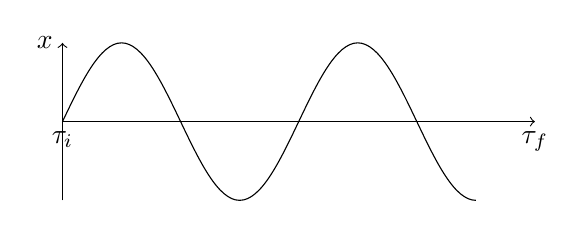
\begin{tikzpicture}
    \draw [->] (0,0) node [below] {$\tau_i$} --++ (6,0) node [below] {$\tau_f$};
    \draw [->] (0,-1) -- (0,1) node [left] {$x$};
    \draw (0,0) sin (.75,1) cos (1.5,0) sin (2.25,-1) cos (3,0)
                sin (3.75,1) cos (4.5,0) sin (5.25,-1);
  \end{tikzpicture}
\end{center}
We can interrupt it with tension $x(\tau)$ and potention $V(x(\tau))$,
completely a classical problem.
So, in the end, $\mathcal L_E$ is the energy density respects to the $\tau$-axis after the translation.
Concerning $S_E$
\[
  S_E[x(\tau)] = \int \d\tau \mathcal L_E(x(t), \dot x(t))
\]
it is of course the total energy after the translation.
In other words, $t$ is replaced by $\tau$.
i.e., in $\mathbb R^{d+1}$,
$d$ is supposed to the space dimension, and one for time.

\subsection{Quantum P.F.}

The partition function is
\begin{equation}
  Z = \Tr \upe^{-\beta\hat H}, \qq{where} \hat H = \frac{\hat p^2}{2m} + V(\hat x)
\end{equation}
where trace can be identity, i.e.,
\[
  Z_n = \int \d x_n \braket<x_0|\upe^{-\beta\hat H}|x_0>
\]
by inserting the identity $\int \d x_0 \ketbra|x_0><x_0| = \identity$.
What we need to do is to compare
\[
  \braket<x_0|\upe^{-\beta\hat H}|x_0> \qq{with}
  \braket<x_f|\hat U(t_f, t_i)|x_i>
\]
by slicing $\beta \sim t_f - t_i$ into $N$ pieces, each segment has a length of
$\delta \tau = \beta/N$. Then
\[
  Z = \int \d x_0 \d x_1 \cdots \d x_{N-1}
      \braket<x_0|\upe^{-\delta\tau\hat H}|x_{N-1}> \cdots
      \braket<x_n|\upe^{-\delta\tau\hat H}|x_{n-1}> \cdots
      \braket<x_1|\upe^{-\delta\tau\hat H}|x_0>
\]
What we have derived is
\[
  \braket<x_n|\upe^{-\frac\iu\hbar\delta t\hat H}|x_{n-1}>
= \ab(\frac{m}{2\pi\iu\hbar\delta t})^{1/2} \upe^{-\frac\iu\hbar \mathcal L(x_n, \dot x_n)\delta t}
\]
simply replace $\frac\iu\hbar\delta t \to \delta \tau$, then
\[
  \braket<x_n|\upe^{-\delta\tau\hat H}|x_{n-1}>
= \ab(\frac m{2\pi\hbar\delta\tau})^{1/2} \upe^{-\mathcal L_E(x(\tau_n), \dot x(\tau_n))\delta\tau}
\]
with the periodic boundary condition $x_N \equiv x_0$,
substitute it back, the partition function becomes
\begin{equation}
  Z = \ab(\frac{m}{2\pi\iu\hbar\delta t})^{N/2} \int \prod_{n=0}^{N-1} \d x_n
  \upe^{-\sum_{n=0}^{N-1} \delta\tau \mathcal L_E(x(\tau_n), \dot x(\tau_n))}
  \xlongequal{N\to\infty} \int_{x(0) = x(f)} \mathcal D x(\tau) \upe^{-S_E[x(\tau)]}
\end{equation}
then the action
\begin{equation}
  S_E[x_\tau] = \int_{0}^\beta \d \tau \mathcal L_E(x(\tau), \dot x(\tau))
\end{equation}

\paragraph{Quiz}

\begin{problem}
  Gaussian Integral
  \[
    \int \d x_1 \d x_2 \upe^{-(x_1,x_2) \begin{psmallmatrix}
      1 & \sfrac12\\\sfrac12 & 1
    \end{psmallmatrix} \begin{psmallmatrix}
      x_1\\x_2
    \end{psmallmatrix}}
  \]
  \rule{\linewidth}{1pt}
  Change the variable $x$ to a vector $\bm x = (x_1, x_2)$, i.e.
  \[
    \int \d\bm x \upe^{-\bm x \cdot \mathbf A \cdot \bm x}
  = \det\ab(\frac{\mathbf A}{\pi})^{-1/2}
  \]
\end{problem}

\begin{problem}
  \[
    F[\pi] = \frac12 \int_{t_i}^{t_f} \d t_1 \d t_2 \phi(t_1) A(t_1,t_2) \phi(t_2)
  \]
  then compute the second derivative $(\delta_\phi^2F)[\eta]$.\\
  \rule{\linewidth}{1pt}
  \[
    (\delta_\phi^2F)[\eta] = 2F[\eta]
  \]
\end{problem}

\begin{problem}
  The Lagrangian
  \[
    L(\phi_t, \dot\phi_t) = a\phi_t^2 + b\dot\phi_t^2 + c\phi_t\dot\phi_t
  \]
  show that $S[\phi] = S[\phi_c] + S[\phi - \phi_c]$,
  where $\phi_c$ is a classical path: $(\delta_\phi S)\big|_{\phi=\phi_c} = 0$.\\
  \rule{\linewidth}{1pt}
  Taylo expansion to $S[x + \eta]$
  \[
    S[x_c + \eta] = S[x] + (\delta_{x_c} S[\eta]) + \frac12(\delta_{x_c}^2S)[\eta]
  = S[x_c] + 0 + S[\eta]
  \]
\end{problem}

\paragraph{Case study}

We start from a Lagrangian
\begin{equation}
  \mathcal L(x(t), \dot x(t)) = \frac12m\dot x^2 - \frac12m\omega^2 x^2
\end{equation}
and we want to compute the propagator
$\int_{x(t_{i,f}) = x_{i,f}} \mathcal D(x) \upe^{\iu S[x(t)]}$.
This computation would be purely quantum.
We choose the staring point: $x(t_{i,f}) = x_{i,f}$.
We separate
\[
  x(t) = x_c(t) + \eta(t)
\]
Since $x_i$ and $x_f$ are fixed, so we get the boundary condition $\eta(t_i) = \eta(t_f) = 0$. Then the action
\[
  S[x_c + \eta]
= \upe^{\iu S[x_c]} \cdot \int_{\eta(t_i) = \eta(t_f) = 0} \mathcal D\eta(t) \upe^{\iu S{[\eta(t)]}}
\]
where $S[x(t)] = S[x_c] + S[\eta_c]$.
\begin{enumext}
  \item Comput $S[x_c]$
  \[
    S[x_c] = \int_{t_i}^{t_f} \d t \mathcal L(x_c(t), \dot x_c(t))
  = \int_{t_i}^{t_f} \mathcal L(t)
  \]
  Concering $x_c(t)$, using the E-L eq. (EOM)
  \[
    \odv*{\pdv{\mathcal L}{\dot x}}t - \pdv{\mathcal L}x = 0, \qq{or}
    (\pdif t^2 + \omega^2) x(t) = 0
  \]
  Before getting the solution, applying the boundary condition
  \[
    x(t_i) = x_i, \qq{and} x(t_f) = x_f
  \]
  The solution would be generally
  \[
    x_c(t) = x_0 \sin(\omega t + \phi_0)
  \]
  where $x_0$ and $\phi_0$ will be fixed by the boundary condition.
  Substitute it into the Lagrangian
  \[
    \mathcal L_{x_c}(t) = \frac12 m\omega^2 x0^2 \cos[2(\omega t + \phi_0)]
  \]
  and the actioin
  \[
    S[x_c] = \frac{m\omega}{2\sin(\omega\Delta t)}
             [(x_i^2 + x_f^2) \cos(\omega\Delta t) - 2x_ix_f]
  \]
  Now, we shall handle
  \[
    \int \mathcal D\eta \upe^{\iu S[\eta]}, \qq{where}
    S[\eta] = \int_{t_i}^{t_f} \d t
              \ab(\frac12 m\dot\eta^2 - \frac12 m\omega^2\eta^2)
  \]
  Referring \textbf{\textsf{Quiz 0.9}},
  $\int \d\bm x \upe^{-\bm x \cdot \mathbf A \bm x}$, we can convert the integral kernel to
  \[
    -\frac12 m\eta (\pdif t^2 + \omega^2) \eta
  \]
  where $(\pdif t^2 + \omega^2)$ is the ``sandwich'' term $\mathbf A$.
  Since
  \[
    \int \d t \dot\eta^2 = \cancel{(\eta\dot\eta)\big|_{t_i}^{t_f}}
  - \int \d t \ddot\eta
  \]
  Then the expression of the action is
  \[
    \int \mathcal D \eta \upe^{\iu S[\eta]}
  = \det\ab(\frac{\mathbf A}{\pi})^{-1/2}
  = \det\ab[\frac{\iu m}{2\pi}(\pdif t^2 + \omega^2)]^{-1/2}
  \]
  Given a matrix $M$, its determent $\det(\mathbf M) = \prod_i \lambda_i$,
  where $\lambda_i$ is the eigenvalue of $\mathbf M$. That is how we interrupt the determine of $\mathbf A$
  \[
    (\pdif t^2 + \omega^2)\psi_n = \lambda_n \psi_n
  \]
  We just define $X$
  \[
    X = \det(\pdif t^2 + \omega^2)
  = \prod_n \lambda_n 
  \]
  we need to solve the ODE by applying the boundary condition $\eta(t_i) = \eta(t_f) = 0$, i.e., $\psi_n(t_i) = \psi_n(t_f) = 0$.
  The eigenvalue
  \[
    \lambda_n = \omega^2 - (n\pi/\Delta t)^2
  = \omega^2- (n\Omega)^2, \quad n = 1, 2, \ldots, \infty
  \]
  and substitute it into $X$
  \[
    X = \prod_n \ab(\omega^2 - n^2\Omega^2)
  \]
  Take the log
  \[
    \ln X = \sum_n \ln(\omega^2 - n^2 \Omega^2)
  \]
  then take the derivative of $\omega$
  \[
    \pdv{\ln X}\omega = \sum_{n=1}^\infty \frac{2\omega}{\omega^2 - n^2\Omega^2}
  = \frac\pi\Omega \cotan \ab(\frac{\pi\omega}{\Omega}) - \frac1\omega
  \]
  integral to both sides
  \[
    \ln X = \ln\ab(\frac{\sin \omega\Delta t}{\omega} + \text{Const})
  \]
  Directly jump to the determine
  \[
    \det(\quad)^{-1/2} = C\ab(\frac{\omega}{\sim(\omega\Delta t)})^{1/2}
  \]
  When $\omega \to 0$, the Lagrangian
  \[
    \mathcal L = \frac12 m\dot x^2
  \]
  which is the free particle, and the determine $\det(\quad)^{-1/2} \sim \Delta t^{-1/2}$.
  For the boundaty condition of the free particle
  \[
    \braket<x=0|\upe^{-\frac\iu\hbar\hat H_0\Delta t}|x=0>
  = \int \d x \braket<x = 0|k> \upe^{-\iu\frac{\hat k^2}{2m} \Delta t}
    \braket<k|x = 0>
  = \frac1{2\pi} \int \d k \upe^{-\iu\frac{k^2}{2m}\Delta t}
  = \ab(\frac{m}{2\pi\iu\Delta t})^{1/2}
  \]
  where $H_0 = \frac{\hat p^2}{2m} = \frac{\hat k^2}{2m}$, set $\hbar = 1$,
  and $\braket<x|k> = \frac1{\sqrt{2\pi}} \upe^{\iu kx}$.
  To infer $C$, comparing the result with the determine
  \[
    \ab(\frac{m}{2\pi\iu\Delta t})^{1/2} = (\Delta)^{-1/2}, \qq{and}
    C = \ab(\frac m{2\pi\iu})^{1/2}
  \]
  Then we get $X$.
  \[
    \psi_n(t) \sim \sin \ab[\frac{n\pi}{\Delta t}(t - t_i)]
  \]
  Then substitute it into the ODE to obtain the normalization constant.
\end{enumext}

\section{PI \& Correlation functions}

Review what we get in the last section
\begin{equation}
  \begin{aligned}
    Z & = \int \d x_0 \upe^{\underset{x_i = x_f = x_0}{\iu S[x_c]}} \ab[\frac{m\omega}{2\pi\iu\sin(\omega t)}]^{1/2}\\
  & = \ab[\frac\pi{\iu m\omega \tan(\omega\Delta t/2)} \cdot
      \frac{m\omega}{2\pi\iu\sin(\Omega\Delta t)}]^{1/2}
    \xlongequal{\Delta \mapsto -\iu\beta}
      \ab[2\sinh\ab(\frac{\beta\omega}{2})]^{-1}
  \end{aligned}
\end{equation}
where the action
\begin{equation}
  S[x_c] = \frac{m\omega}{2\sin\omega\Delta t}
            [(x_i^2 + x_f^2) \cos(\omega\Delta t) - 2x_ix_f]
  \xlongequal{x_i=x_f=x_0} -\ab(m\omega \tan\frac{\omega\Delta t}{2}) x_0^2
\end{equation}
Two key points we need to keep in mind
\begin{itemize}
  \item The time interval $\Delta t \equiv t_f - t_i$,
  from the dictionary (Wick rotation) $t \mapsto -\iu\tau$,
  then $\Delta t \mapsto -\iu\beta$.
  \item The periodic boundary condition $x_i = x_f = x_0$.
\end{itemize}
The partition function should be like
\begin{equation}
  Z = \Tr\ab[\upe^{-\beta\omega\ab(\hat n+\frac12)}]
= \sum_{n=0}^\infty \upe^{-\beta\omega\ab(n+\frac12)}
= \frac{\upe^{-\beta\omega/2}}{1 - \upe^{-\beta\omega}}
  \equiv \ab[2\sinh\ab(\frac{\beta\omega}{2})]^{-1}
\end{equation}
where we have two context
\begin{enumext}
  \item Quantum mechaincs context $\braket<x_f|\hat U(t_f, t_i)|x_i>$
  \item Statistics mechanics context
\end{enumext}
\hrule
The path integration
\[
  \frac ZZ = \sum_{\underset{\text{configuration}}{\phi}} \frac{\rho[\phi]}{Z}
\]
where $\rho$ is so-called the raw probability, and $\rho[\phi]/Z$ is the actual probability.
Distinguish $\upe^{\iu S}$, $\upe^{-S_E}$, $\upe^{\beta H}$.
\begin{center}
  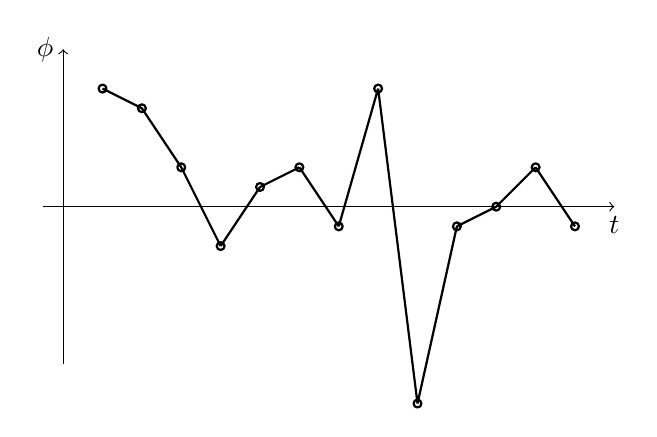
\begin{tikzpicture}[xscale = .5]
    \draw [->] (-.5,0) -- (14,0) node [below] {$t$};
    \draw [->] (0,-2) -- (0,2) node [left] {$\phi$};
    \draw [thick, rounded corners = .5cm, line join = round]
      (1,1.5) ellipse (.1 and .05) -- (2,1.25) ellipse (.1 and .05) --
      (3,.5)  ellipse (.1 and .05) -- (4,-.5)  ellipse (.1 and .05) --
      (5,.25)  ellipse (.1 and .05) -- (6,.5)  ellipse (.1 and .05) --
      (7,-.25) ellipse (.1 and .05) -- (8,1.5) ellipse (.1 and .05) --
      (9,-2.5) ellipse (.1 and .05) -- (10,-.25) ellipse (.1 and .05) --
      (11,0)   ellipse (.1 and .05) -- (12,.5) ellipse (.1 and .05) --
      (13,-.25) ellipse (.1 and .05);
  \end{tikzpicture}
\end{center}
If one measure for many tims, he may get something like a curve.
\[
  \frac1N \sum_i \phi_i \xlongequal{N\to\infty} \braket<\phi>
= \int \d\phi(\phi)\phi
\]
and
\[
  \frac1N \sum_i \phi_i = \braket<\phi^2> = \int \d\phi p(\phi)\phi^2z \phi^2
\]
and we call $\braket<\hat \phi>$, $n$-th moments. The variance
\[
  (\phi - \braket<\phi>)^2 = \braket<\phi>^2 - \braket<\phi^2>
\]
Caldular $\phi$
\begin{align}
  \braket<\phi^2>^d = \braket<\phi - \phi>^3, \qq{cumulants}
  \braket<\phi>^3 = \braket<\phi^3> - \braket<\phi>^3
\end{align}
Computing $\braket<\phi_i, \phi_j>$, where $i$ and $j$ can be treated as
different time. We define
\begin{equation}
  \frac1{N_\phi}\sum_{\phi(t)} \phi_i \phi_j = \braket<\phi_i \phi_j>
= \int\mathcal D\phi p[\phi] \cdot \phi_i \phi_j
\end{equation}
$N_\phi$ means how many times we take the sequence.
Means integrating with all the configurations. This is the correlation function we are talking about.

What we care about more is $\frac1N \sum_i \phi_i \phi_{i+\delta}$ instead the specific $i$ and $j$.

We can also expand to
\[
  \braket<\phi_i\phi_j\cdots\phi_n>
= \braket<\phi_i\phi_j\cdots\phi_n> -
  (a\braket<\phi_i>\braket<\phi_i\phi_j\cdots\phi_n>
+ b\braket<\phi_i\phi_j>\braket<\phi_i\phi_j\cdots\phi_n> + \cdots +
  c\braket<\phi_i> \braket<\phi_j> \cdots \braket<\phi_n>)
\]

\subsection{Generating Function(al) SI Partition Function}

\paragraph{Generating Function}

The set
\[
  \{m_0, m_1, m_2, m_3, \cdots\}
\]
We introduce a function of auxiliary variable $a$
\begin{equation}
  f(a) = m_0 + m_1a + \frac12m_2a^2 + \frac1{3!} m_3a^3 + \cdots
= \sum_{n=0}^\infty \frac1{n!} m_n a^n
\end{equation}
We just let the set of numbers as the series coefficients. In the end, we have
\[
  C_n = \odv[n]fa \bigg|_{a=0}
\]
and we treat $m_n$ as
\begin{equation}
  m_n = \braket<\phi^n> = \int\d\phi p(\phi) \phi^n
\end{equation}
Then, $f(a)$ becomes
\begin{equation}
  f_m(a) = \sum_n \frac1{n!} a^n \int \d\phi p(\phi)\phi^n
= \int\d\phi p(\phi) \upe^{a\phi} = \braket<\upe^{a\phi}>, \quad
  f_c(a) = \ln f_m(a)
\end{equation}
where $m_0 = 1$.
\begin{align*}
  K_0 & = f_c(0) = \ln f_m(0) = \ln m_0 = 0,\\
  K_1 & = \odv{f_C(a)}a \bigg|_{a=0}
= \frac1{f_m(0)} \odv{f_m(a)}a \bigg|_{a=0} = m_1,\\
  K_2 & = \odv[2]{f_C(a)}a\bigg|_{a=0} = \frac{f''_m(a) f_m(a) - f'_m(a) f_m'(a)}{f_m^2(a)}\bigg|_{a=0}
= m_2 - m_1^2 = \braket<\phi^2> - \braket<\phi>^2\\
  K_3 & = \odv*[fun]{\frac{f_m'}{f_m} - \ab(\frac{f_m'}{f_m})^2}a
= \frac{f_m^{(3)}f_m - f_m''f_m'}{f_m^2} - 2\frac{f_m'}{f_m} \frac{f_m''f_m - f_m'f_m'}{f_m^2}\bigg|_{a=0}\\
& = m_3 - 3m_2m_1 + 2m_1^3 = \braket<\phi^3> - 3\braket<\phi^2>\braket<\phi> + 2\braket<\phi>^3
\end{align*}

\paragraph{Generating Function\textcolor{red}{al}}

\begin{center}
  \begin{tabular}{llll}
    \toprule
    Function    & $f(\phi)$    & single variable             & $\phi$\\
    Functional  & $F[\phi(t)]$ & multiple variable / vector  & $\{\phi_i\}$\\
                &           & continous variables         & $\phi(t)$ (function)\\
    \bottomrule
  \end{tabular}
\end{center}

Now the coefficients set becomes
\[
  \{C_0,\ C_1(x),\ C_2(x_1,x_2),\ \ldots\,,~C_n(x_1,\ x_2,\ \ldots\,,~x_n),\ \ldots\}
\]
Then the auxiliary function is $a(x)$
\begin{multline}
  F[a(x)] = C_0 + \int \d x_1 C_1(x_1) a(x_1)
      + \frac1{2!} \int\d x_1\d x_2 C_2(x_1x_2) a(x_1)a(x_2) + \cdots\\
      + \frac1{n!} \int \d x_1 \cdots \d x_n C_n(x_1,\ x_2,\ \ldots\,,~x_n)
        a(x_1) a(x_2) \cdots a(x_n)
\end{multline}
Each term here to the $n$-th order is we used to call the functional derivative $(\delta^nF)[a]$.
Considering $C_n$
\[
  C_n(x_1,\ x_2,\ \ldots\,,~x_n) \sim
  \braket<\phi(x_1) \phi(x_2) \cdots \phi(x_n)>
= \fdv{F^n[a]}{a(x_1), a(x_2), \cdots, a(x_n)}\bigg|_{a=0}
\]
\begin{framed}
  Someone hasn't understand functional (derivative) NOW!!!

  $a = (a_1, a_2)$, $\phi = (\phi_1, \phi_1)$.
  \[
    F[a] = a_1\phi_1 + a_2\phi_2 = \sum_{i=1}^2 a_i\phi_i = a^{\mathsf T}\phi
  \]
  \[
    C_{i=1,2}^{(1)} = \fdv F{a_{1,2}} = \phi_{1,2}, \quad
    C_{ij}^{(2)} = \fdv[2]F{a_i,a_j},
  \]
  or more complex
  \[
    F[a] = (a_1, a_2) \mathbf A_{2\times 2} \begin{pmatrix}
      a_1\\a_2
    \end{pmatrix} = a^{\mathsf T}\mathbf A a
  \]
\end{framed}

\paragraph{Quiz}
\begin{example}
  \[
    C_n(x_1,\ x_2,\ \ldots\,,~x_n) = \braket<\phi(x_1) \phi(x_2) \cdots \phi(x_n)>
  = \int \mathcal D\phi p[\phi] \phi(x_1) \phi(x_2) \cdots \phi(x_n)
  \]
  Calculate the generating function $F[a(x)]$ first.
  \[
    F[a(x)] = \int \mathcal D\phi p[\phi] \upe^{\int \d x a(x) p(x)}
  = \braket*\big<\upe^{a^{\mathsf T}\phi}>
  \]
  Consider $p[\phi]/Z$, $Z = \int\mathcal D\phi p[\phi]$,
  where $p[\phi] = \upe^{-S_E[p]}$.
  Write $F[a(x)]$ explicitly
  \[
    F[a(x)] \xlongequal{p[\phi]=\upe^{-S[\phi]}/Z} \frac1Z
    \underbrace{\int \mathcal D\phi \upe^{-\frac{S[\phi]-a^{\mathsf T}\phi}{S_a[\phi]}}}_{Z_a}
  = \frac{Z_a}{Z_0}
  \]
  where $a$ is the \emph{control variable},
  and $\phi$ is the \emph{system variable}.
  $Z_a$ can be $Z_a(\mathbf H, \mathbf m)$ or $Z_a(\mathbf A, \mathbf j)$.
  \[
    \pdv{\braket<m(x_1)>}{h(x_2)}\bigg|_{h=0}
  = \fdv*[fun]{\fdv{F[h]}{h(x_1)}}{h(x_2)} = \braket<m(x_1) m(x_2)>|_{h=0}
  \]
  In contrast, $h$ is $a$, $m$ is $\phi$. It's what we called the \emph{susceptibility}, or \emph{linear response function}.
\end{example}

\begin{example}
  Action function $S[\phi] = \frac12 \phi^{\mathsf T} A\phi$.
  Calculate $\braket<\phi_i, \phi_j>$.
  \[
    Z_a = \int \mathcal D\phi \upe^{-S[\phi]+a^{\mathsf T}\phi}
  = \int\mathcal D\phi \upe^{-\frac12\phi^{\mathsf T}A\phi + a^{\mathsf T\phi}}
  = \det\ab(2\pi\mathbf A^{-1})^{1/2} \upe^{a^{\mathsf T}\mathbf A^{-1}a/2},
    \quad
    Z_0 = Z_a\big|_{a=0}.
  \]
  and $Z_0$ is just the Gaussian term.
  \[  
  F[a] = \frac{Z_a}{Z_0} = \upe^{a^{\mathsf T}\mathbf A^{-1}a/2}
  \]
  Define $\mathbf A^{-1} = G$, matsubara Green function.
  \[
    \braket<\phi_i\phi_j> = \pdv F{a_i, a_j}\bigg|_{a=0}
  = G_{ij}
  \]
\end{example}

\paragraph{Quiz 8}

Make a sentense with the following phrases:

\textbf{Path Integral}
\textbf{Partition Function} (is)
\textbf{Generating Functional} (of)
\textbf{Correlation Functions}

and combine them with ``is'', ``are'', ``of'', ``at'', ``on'', ``in'', ``below'', ``above'', etc.

DeepSeek: The Path Integral formulation of quantum mechanics reveals that the Partition Function is a specific type of Generating Functional, from which all Correlation Functions can be derived by taking functional derivatives."

\paragraph{Explanation}

The partition function
\[
  Z = \sum_n \upe^{-\beta E_n}
\]
is a kind of generating function, i.e., we want the average and the fluctuation of energy
\[
  \braket<E>, \qq{and} \braket<E^2> - \braket<E>^2
\]
So, the Generating function for energy is, for momentum, we try to evalute
\[
  f_m(a) = \braket<\upe^{aE}> = \frac1{Z_0} \underbrace{\sum_n \upe^{(a-\beta) E_n}}_{Z_a} = \frac{Z_a}{Z_0}
\]
Then, the critical generating function
\[
  f_c = \ln f_m(a) = \ln Z_a - \ln Z_0
\]
Since $\braket<E^2>^c = \braket<E^2> - \braket<E>^2$, then the cumulent
\[
  \braket<E>^c = \braket<E> = \odv*{f_c(a)}a \bigg|_{a=0}
= \odv{\ln Z}a \bigg|_{a=0} = -\odv{\ln Z}\beta
\]
By construction, the cumulent
\[
  \braket<E^2>^c = \braket<E^2> - \braket<E>^2 = \odv[2]{f_C(a)}a\bigg|_{a=0}
= \odv[2]{\ln Z}\beta
\equiv \frac{\beta^2}{k_B}C_v
\]
\rule \linewidth {.5pt}
In the new context, upgrade to ``functional'': consider the general form of the
partition function
\[
  \mathcal Z = \int \mathcal D\phi(\tau) \upe^{-\mathcal S_E[\phi]}
\]
we integrate over all the configuration, since they are very complicated, so we
use the ``fancy'' expression.

Starting from the $n$-point correlation function
\[
  \braket<\phi(\tau_1) \phi(\tau_2) \cdots \phi(\tau_n)>
  \xlongequal{\text{variables are continous}}
  \braket<\phi_i \phi_j \cdots \phi_l>^{(c)} =
  \pdv[n-3]{F_{m,c}[a]}{a_i, a_j, \cdots, a_l} \bigg|_{a=0}
\]
and the definition of $F_m[a]$ is
\[
  F_m[a] = \braket<e^{a\tran\phi}>
= \frac1Z \int \mathcal D\phi
  \upe^{-S_E + \underset{\text{`source' term}}{\underline{a\tran\phi}}}
= \frac{Z_a}{Z_0}
\]
where we take $Z_a = \upe^{-S_a}$ and $S_a = S_E - a\tran\phi$.
The term $a\tran\phi = \phi\tran a$ is symmetric, can be expressed as
\[
  a\tran\phi = \int \d\tau a(\tau) \phi(\tau) \sim \sum_i a_i \phi_i
\]
and critical one is $F_c[a] \sim \ln Z_a$.

Then the fluctuation
\[
  \braket<\phi_i\phi_j>^c
= \braket<\phi_i\phi_j> - \braket<\phi_i>\braket<\phi_j>.
\]
Define
\[
  (\chi_\phi)_{ij} = \pdv{\braket<\phi_i>_a}{a_j}\bigg|_{a=0}
= \pdv*{\pdv{F_c[a]}{a_i}}{a_j} \bigg|_{a=0}
= \pdv{\ln Z_a}{a_i a_j} \bigg|_{a=0} \equiv \braket<\phi_i\phi_j>^c
\]
This relation, is so-called the \emph{Fluctuation-Dissipation Theorem}.

\section{Green's Function}

Consider
\[
  S_{E, \text{or} a}[\phi] = \frac12 \phi\tran A\phi - a\tran\phi
\]
which is the same format of $S_a = S_0 - a\tran\phi$, and $A$ is symmetric,
$A = A\tran$.
Here,
\[
  \phi\tran A\phi = \sum_{ij} A_{ij} \phi_i \phi_j
= \int \d\tau \d\tau' A(\tau, \tau') \phi(\tau) \phi(\tau')
\]
$A$ is symmetric. Then,
\[
  F_m[a] = \frac{Z_a}{Z_0}
= \frac{\int\mathcal D\phi \upe^{-S_a}}{\int \mathcal D\phi \upe^{-S_0}}
= \upe^{\frac12 a\tran A^{-1} a}
\]
we define the Green's function is the inverse
\begin{equation}
  G \equiv A^{-1}, \qq{or} AG = \identity
\end{equation}
Rewrite it
\[
  \sum_j A_{ij} G_{jl} = \delta_{il}
\]
make it continuous
\[
  \int \d\tau A(\tau_1, \tau) G(\tau, \tau_2) = \delta(\tau_1 - \tau_2)
\]
The propagator $\braket<x_f|\hat U(t_f,t_i)|x_i>$ can be just what Green's
function is. The EOM here can be
\[
  \delta\phi S_a = 0
\]
\begin{enumext}
  \item then we have
  \[
    \delta\phi S_a[\eta]
  = \odv{S[\phi + \epsilon\eta]}\epsilon\bigg|_{\epsilon=0}
  = \frac12(\eta\tran A\phi + \phi\tran A\eta) - a\tran\eta
  \xlongequal[a\tran\eta=\eta\tran a]{\phi\tran A\eta = \eta\tran A\phi}
    \eta\tran(A\phi - a)
  \]
  The solution is
  \[
    A\phi = a, \qq{exist} A\phi_0, \qq{then}
    \phi_c = A^{-1}a + \phi_0 \xlongequal{G\equiv A^{-1}} Ga + \phi_0
  \]
  where $G$ can be a matrix, $a$ can be a vector. Now, $\phi_c(\tau)$ can be
  \[
    \phi_c(\tau) = \int \d\tau'
    \underset{\text{propagator}}{\underline{G(\tau, \tau')}} \,
    \underset{\text{source}}{\underline{a(\tau')}} + \phi_0(\tau)
  \]
  the source $a(\tau)$ can be charge distribution,
  $\phi$ can be the field propagated by the charge.
  \item The functional derivative
  \[
    \fdv{S_a[\phi]}{\phi_i} = \sum_j A_{ij} \phi_j - a_i = 0
  \]
  since $\sum_{jl} A_{jl} \phi_j \phi_l = \phi\tran A\phi$ and
  $a\tran\phi = \sum_j a_j\phi_j$.
\end{enumext}

\paragraph{Case study: Quantum Harmonic Oscillator}

The Hamiltonian ($\hbar = 0$)
\[
  \hat H = \frac{\hat k^2}{2m} + \frac12m\omega^2\hat x^2
\]
which is basically the Canonical Quantization.
Then, we can write down the Path Integral form. We need the Lagrangian
\[
  \mathcal L(x(t), \dot x(t)) = \frac12 m(\dot x^2 - \omega^2x^2)
\]
The action is a functional of
\[
  \mathcal S[x(t)] = \int_{t_i}^{t_f} \d t \mathcal L(x, \dot x)
= -\int_{t_i}^{t_f} \d t \frac12mx(t) (\pdif t^2 + \omega^2) x(t)
  +S_\text{boundary term}
\]
The $S_\text{boundary term}$ is due to ``integral by part''.
Therefore
\[
  \mathcal Z = \int \mathcal D x\upe^{\iu\mathcal S[x]}
\]
one can let $\iu t \leftrightarrow \tau$.
The Wick rotation version can be $\iu\mathcal S \leftrightarrow -S_E$,
and the Euclidian version can be
$S \leftrightarrow S_E = \int_0^\beta \d\tau \mathcal L_E(x(\tau), \dot x(\tau))$,
and the boundary term does not appear here.
\[
  S_E = \int_0^\beta \d\tau \mathcal L_E(x(\tau), \dot x(\tau))
= \int_0^\beta \d\tau \frac12 mx(\tau) (\omega^2 - \pdif\tau^2) x(\tau)
\]
$\phi(\tau)$ is now replaced by $x(\tau)$, i.e.,
\[
  \frac12 x\tran A x = \frac12 \int_0^\beta \d\tau \int_0^\beta\d\tau'
  x(\tau) A(\tau,\tau') x(\tau')
\]
If we insert the identity $\int_0^\beta\d\tau' \delta(\tau - \tau')$,
then, we will have a prime for the first $x$, i.e.,
\[
  S_E = \int_0^\beta \d\tau \int_0^\beta \d\tau' \delta(\tau - \tau')
        \frac12 mx(\tau) (\omega^2 - \pdif\tau^2) x(\tau)
\]
Therefore, $A$ will be
\[
  A(\tau', \tau) = m\delta(\tau' - \tau) (\omega^2 - \pdif\tau^2)
\]
So, finally, we can use
\begin{equation}
  \int \d\tau A(\tau_1, \tau) G(\tau, \tau_2) = \delta(\tau_1 - \tau_2)
\end{equation}
to generate the Green's funciton.
\[
  \text{LHS} = \int \d\tau \delta(\tau_1 - \tau)
               [m(\omega^2 - \pdif \tau^2)] G(\tau, \tau_2)
= m(\omega^2 - \pdif{\tau_1}^2) G(\tau_1 - \tau_2)
= \delta(\tau_1 - \tau_2) = \text{RHS}
\]
Denote $\Delta\tau = \tau_1 - \tau_2$, then
\[
  \text{LHS} = m(\omega^2 - \pdif{\Delta_\tau}^2) G(\Delta\tau)
= \delta(\Delta\tau) = \text{RHS}
\]
and $G$ satisfies the periodic boundary condition
\[
  G(\Delta\tau) = G(\Delta\tau + \beta).
\]
means that if we have a range, $\tau \in [0, \beta]$,
and the fourier transform
\[
  \ab\{f_l(\tau) = \frac1{\sqrt\beta} \upe^{\iu\frac{2\pi}{\beta} l\tau}\}
\]
where $l \in \mathbb Z$ is a label.
Such that $G(\Delta\tau)$ can be expanded over this space
\begin{equation}
  G(\Delta\tau)
= \sum_l g_l \ab(\frac1{\sqrt\beta} \upe^{\iu\omega_l\Delta\tau})
\end{equation}
where we denote $\omega_l \equiv \frac{2\pi}{\beta}l$.
Then, the left hand side
\[
  \text{LHS} = \sum_l g_l m(\omega^2 + \omega_l^2)
  \ab(\frac1{\sqrt\beta} \upe^{\iu\omega_l \Delta\tau})
\]
Since the $\delta$-function, the right hand side
\[
  \text{RHS} = \delta(\Delta\tau)
= \sum_l \ab(\frac1{\sqrt\beta} \upe^{\iu\omega_l\Delta\tau}) \frac1{\sqrt\beta}
\]
which satisfies the orthogonality
\[
  \sum_l \ab(\frac1{\sqrt\beta} \upe^{\iu\omega_l\tau_2})^*
         \ab(\frac1{\sqrt\beta} \upe^{\iu\omega_l\tau_1})
= \sum_l \frac1\beta \upe^{\iu\omega_l\Delta\tau} = \delta(\Delta\tau)
\]
then, we will derive the coefficient
\[
  g_l = \frac1{\sqrt\beta} \frac{1}{m(\omega^2 + \omega_C^2)}
\]
Therefore, the Green's function, or the correlation function, is
\begin{equation}
  \braket<x(\tau_1) x(\tau_2)> =
  G(\Delta\tau) = \sum_l \frac1\beta
                  \frac{\upe^{\iu\omega_l\Delta\tau}}{m(\omega^2 + \omega_l^2)}
= \frac1{2\pi m} \int_{-\infty}^\infty \d\Omega
  \frac{\upe^{\iu\Omega\Delta t}}{\omega^2 + \Omega^2}
= \frac{\upe^{-\omega|\Delta\tau|}}{2\pi m}.
\end{equation}
where we denote $\omega \to \Omega$ when ground state $T\to0$, $\beta\to\infty$.
In order to obtain the compact form, consider when $\Delta\tau$ is larger/less
than zero, we need to use the Heavisine step function
\begin{equation}
  \braket<x(\tau_1) x(\tau_2)> = G(\Delta\tau)
= \theta(+\Delta\tau) \frac{\upe^{-\omega\Delta\tau}}{2m\omega}
+ \theta(-\Delta\tau) \frac{\upe^{\omega\Delta\tau}}{2m\omega}
\end{equation}
To do the Wick rotation, let $\Delta\tau \leftrightarrow \iu\Delta t$.
Then, $\theta(\Delta\tau) \leftrightarrow \theta(\Delta t)$,
$\iu G(\Delta\tau) \leftrightarrow G(\iu\Delta t)$, i.e., the
\emph{time-ordered Green's function} (in real time)
\begin{equation}
  G(\Delta t) = \theta(+\Delta t) \frac{\iu\upe^{-\iu\omega\Delta t}}{2m\omega}
              + \theta(-\Delta t) \frac{\iu\upe^{+\iu\omega\Delta t}}{2m\omega}
              = G^\text{ret}(\Delta t) + G^\text{adv}(\Delta t)
\end{equation}
and $\braket<x(\tau_1)x(\tau_2)> = \braket<x(\tau_2)x(\tau_1)>$.
To make it symmetric,
\begin{equation}
  \braket<\mathcal T \hat x(t_1) \hat x(t_2)>
= \underbrace{\theta(t_1 - t_2) \braket<\hat x(t_1) \hat x(t_2)>}_
  \text{operator definition of the Retarded Green functioin} +
  \underbrace{\theta(t_2 - t_1) \braket<\hat x(t_2) \hat x(t_1)>}_
  \text{operator definition of the Advanced Green functioin}
\end{equation}
where $\hat x(t) = \upe^{\iu\hat H t} \hat x\upe^{-\iu\hat H t}$.
To accurate it, consider the first term with respect to the ground state
\begin{align*}
    \iu\braket<0|\hat x(t_1) \hat x(t_2)|0>_{t_1>t_2} &
  = \iu\braket<0|
    \upe^{\iu\hat H t_1}\hat x \upe^{-\iu\hat H(t_1-t_2)}\hat x
    \upe^{-\iu\hat Ht_2}|0>
  = \iu \upe^{\iu(\frac12\omega)\Delta t}
    \braket<0|\hat x \upe^{-\iu\hat H\Delta t}\hat x|0>\\
& = \frac\iu{2m\omega} \upe^{\iu(\frac12\omega)\Delta t}
    \braket<1|\upe^{-\iu\hat H\Delta t}|1>
  = \frac\iu{2m\omega} \upe^{+\iu\ab(\frac12\omega)\Delta t}
                       \upe^{-\iu\ab(\frac32\omega)\Delta t}
\end{align*}
where $\hat H\ket|0> = \ab(\frac12\omega)\ket|0>$,
$\Delta t \equiv t_1 - t_2$, and
$\hat x = \frac1{\sqrt{2m\omega}}(\hat a + \hat a^\dagger)$.
Now, go back to the Formalism.

\noindent \rule \linewidth {1pt}

\paragraph{Wick Theorem}

Consider
\[
  \mathcal S[\phi] = \frac12\phi\tran A\phi
\]
and
\[
  \braket<\phi_i\phi_j \cdots\phi_l>
= \fdv[order = n-3, fun]{Z_a/Z_0}{a_i, a_j, ..., a_l}\bigg|_{a=0}
\]
apply Taylor-expansion to the factor
\[
  Z_a/Z_0 = \upe^{\frac12a\tran G a}
= 1 + \ab(\frac12a\tran Ga) + \frac1{2!}\ab(\frac12a\tran Ga)^2 + \cdots
+ \frac1{n!}\ab(\frac12a\tran Ga)^n + \cdots
\]
we denote $n$: $\underbrace{\braket<\phi_i\phi_j \cdots\phi_l>}_n$.
\begin{enumext}
  \item If $n$ is odd, then $\braket<\phi_i\phi_j \cdots\phi_l> = 0$.
  \item If $n$ is even, or let $n = 2n$,
  for any term contains the order of $a$ larger than the order of derivative,
  then this term will vanish since we take $a = 0$.
  Expand the secoond term
  \[
    (a\tran Ga)(a\tran Ga)
  = \ab(\sum_{i_1j_1} a_{i_1} G_{i_1j_1} a_{j_1})
    \ab(\sum_{i_2j_2} a_{i_2} G_{i_2j_2} a_{j_2})
  \]
  then
  \[
    \underbrace{\braket<\phi_i\phi_j \cdots \phi_l>}_{2n}
  = \sum_{(\quad)} (\quad) \underbrace{
    \overbrace{G_{i_1j_1}G_{i_2j_2}}^{\braket<\phi_{i_1}\phi_{j_1}>}
    \cdots G_{i_nj_n}}_n
  \]
  Let the labels $i\to\tau_1$, $j\to\tau_2$, \ldots, $l\to\tau_{2n}$.
  The map can be visualization as
  \begin{center}
    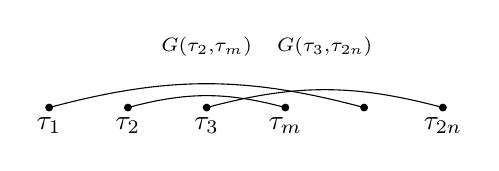
\begin{tikzpicture}
      \fill (1,0) circle (.05) node [below] {$\tau_1$};
      \fill (2,0) circle (.05) node [below] {$\tau_2$};
      \fill (3,0) circle (.05) node [below] {$\tau_3$};
      \fill (5,0) circle (.05);
      \fill (4,0) circle (.05) node [below] {$\tau_m$};
      \fill (6,0) circle (.05) node [below] {$\tau_{2n}$};
      \draw (1,0) to [bend left = 15] (5,0);
      \draw (2,0) to [bend left = 15] (4,0)
       node [above] at (3,15pt) {$\scriptstyle G(\tau_2, \tau_m)$};
      \draw (3,0) to [bend left = 15] (6,0)
       node [above] at (4.5,15pt) {$\scriptstyle G(\tau_3, \tau_{2n})$};
    \end{tikzpicture}
  \end{center}
  The accumulant version is
  \[
    \braket<\underbrace{\phi_i \cdots \phi_l}_n>^c
  = \fdv*[n]{\ab(\frac12a\tran Ga)}{a_i, ..., a_l}
  \]
\end{enumext}

\dbend
\begin{framed}
  Add the interaction term, i.e.,
  \[
    \mathcal S[\phi] = \frac12\phi\tran A\phi + \frac\lambda{4!} \phi^4
  \]
  $S_\text{int}$ is a functional of $\phi$
  \[
    S_\text{int} = \frac\lambda{4!} \phi^4 \sim
    \int \d\tau \phi^4(\tau)
  \]
  compare this guy maybe more general
  \[
    \int \d\tau_1 \d\tau_2 \d\tau_3 \d\tau_4
    A(\tau_1\tau_2\tau_3\tau_4)
    \phi(\tau_1) \phi(\tau_2) \phi(\tau_3) \phi(\tau_4)
  \]
  By Taylor expansion
  \[
    \upe^{-\sin t} = 1 + \frac\lambda{4!}\braket<\phi^4>
                   + \frac1{2!}\ab(\frac\lambda{4!}\braket<\phi^4>)^2 + \cdots
  \]
  Since $Z \to \int\mathcal D\phi\upe^{-S\Delta\tau}(\qquad)$
  and $Z_\text{int} \sim \braket<\upe^{-\sin t}>_0$,
  all the four point becomes
  \begin{align*}
    \begin{tikzpicture}[baseline = (a1.base)]
      \begin{feynhand}
        \vertex [dot] (a1) at (0,0) {};
        \vertex [dot] (b1) at (1,0) {};
        \vertex [dot] (c1) at (2,0) {};
        \vertex [dot] (d1) at (3,0) {};
        \propag       (a1) to [out = 90, in = 90] (b1);
        \propag       (c1) to [out = 90, in = 90] (d1);
      \end{feynhand}
    \end{tikzpicture}
    & \qq{$\longrightarrow$} 8\\
    \begin{tikzpicture}[baseline = (a2.base)]
      \begin{feynhand}
        \vertex [dot] (a2) at (0,0) {};
        \vertex [dot] (b2) at (1,0) {};
        \vertex [dot] (c2) at (2,0) {};
        \vertex [dot] (d2) at (3,0) {};
        \propag       (a2) to [out = 90, in = 90] (c2);
        \propag       (b2) to [out = 90, in = 90] (d2);
      \end{feynhand}
    \end{tikzpicture}
    & \qq{$\longrightarrow$} \infty\\
    \begin{tikzpicture}[baseline = (a3.base)]
      \begin{feynhand}
        \vertex [dot] (a3) at (0,0) {};
        \vertex [dot] (b3) at (1,0) {};
        \vertex [dot] (c3) at (2,0) {};
        \vertex [dot] (d3) at (3,0) {};
        \propag       (a3) to [out = 90, in = 90] (d3);
        \propag       (b3) to [out = 90, in = 90] (c3);
      \end{feynhand}
    \end{tikzpicture}
    & \qq{$\longrightarrow$} ?
  \end{align*}
  i.e., the core of Feynmann diagram.
\end{framed}